% Options for packages loaded elsewhere
\PassOptionsToPackage{unicode}{hyperref}
\PassOptionsToPackage{hyphens}{url}
\PassOptionsToPackage{dvipsnames,svgnames,x11names}{xcolor}
%
\documentclass[
  ignorenonframetext,
  aspectratio=169]{beamer}
\usepackage{pgfpages}
\setbeamertemplate{caption}[numbered]
\setbeamertemplate{caption label separator}{: }
\setbeamercolor{caption name}{fg=normal text.fg}
\beamertemplatenavigationsymbolsempty
% Prevent slide breaks in the middle of a paragraph
\widowpenalties 1 10000
\raggedbottom
\setbeamertemplate{part page}{
  \centering
  \begin{beamercolorbox}[sep=16pt,center]{part title}
    \usebeamerfont{part title}\insertpart\par
  \end{beamercolorbox}
}
\setbeamertemplate{section page}{
  \centering
  \begin{beamercolorbox}[sep=12pt,center]{part title}
    \usebeamerfont{section title}\insertsection\par
  \end{beamercolorbox}
}
\setbeamertemplate{subsection page}{
  \centering
  \begin{beamercolorbox}[sep=8pt,center]{part title}
    \usebeamerfont{subsection title}\insertsubsection\par
  \end{beamercolorbox}
}
\AtBeginPart{
  \frame{\partpage}
}
\AtBeginSection{
  \ifbibliography
  \else
    \frame{\sectionpage}
  \fi
}
\AtBeginSubsection{
  \frame{\subsectionpage}
}
\usepackage{amsmath,amssymb}
\usepackage{lmodern}
\usepackage{iftex}
\ifPDFTeX
  \usepackage[T1]{fontenc}
  \usepackage[utf8]{inputenc}
  \usepackage{textcomp} % provide euro and other symbols
\else % if luatex or xetex
  \usepackage{unicode-math}
  \defaultfontfeatures{Scale=MatchLowercase}
  \defaultfontfeatures[\rmfamily]{Ligatures=TeX,Scale=1}
\fi
\usetheme[]{CambridgeUS}
% Use upquote if available, for straight quotes in verbatim environments
\IfFileExists{upquote.sty}{\usepackage{upquote}}{}
\IfFileExists{microtype.sty}{% use microtype if available
  \usepackage[]{microtype}
  \UseMicrotypeSet[protrusion]{basicmath} % disable protrusion for tt fonts
}{}
\makeatletter
\@ifundefined{KOMAClassName}{% if non-KOMA class
  \IfFileExists{parskip.sty}{%
    \usepackage{parskip}
  }{% else
    \setlength{\parindent}{0pt}
    \setlength{\parskip}{6pt plus 2pt minus 1pt}}
}{% if KOMA class
  \KOMAoptions{parskip=half}}
\makeatother
\usepackage{xcolor}
\newif\ifbibliography
\usepackage{color}
\usepackage{fancyvrb}
\newcommand{\VerbBar}{|}
\newcommand{\VERB}{\Verb[commandchars=\\\{\}]}
\DefineVerbatimEnvironment{Highlighting}{Verbatim}{commandchars=\\\{\}}
% Add ',fontsize=\small' for more characters per line
\usepackage{framed}
\definecolor{shadecolor}{RGB}{248,248,248}
\newenvironment{Shaded}{\begin{snugshade}}{\end{snugshade}}
\newcommand{\AlertTok}[1]{\textcolor[rgb]{0.94,0.16,0.16}{#1}}
\newcommand{\AnnotationTok}[1]{\textcolor[rgb]{0.56,0.35,0.01}{\textbf{\textit{#1}}}}
\newcommand{\AttributeTok}[1]{\textcolor[rgb]{0.77,0.63,0.00}{#1}}
\newcommand{\BaseNTok}[1]{\textcolor[rgb]{0.00,0.00,0.81}{#1}}
\newcommand{\BuiltInTok}[1]{#1}
\newcommand{\CharTok}[1]{\textcolor[rgb]{0.31,0.60,0.02}{#1}}
\newcommand{\CommentTok}[1]{\textcolor[rgb]{0.56,0.35,0.01}{\textit{#1}}}
\newcommand{\CommentVarTok}[1]{\textcolor[rgb]{0.56,0.35,0.01}{\textbf{\textit{#1}}}}
\newcommand{\ConstantTok}[1]{\textcolor[rgb]{0.00,0.00,0.00}{#1}}
\newcommand{\ControlFlowTok}[1]{\textcolor[rgb]{0.13,0.29,0.53}{\textbf{#1}}}
\newcommand{\DataTypeTok}[1]{\textcolor[rgb]{0.13,0.29,0.53}{#1}}
\newcommand{\DecValTok}[1]{\textcolor[rgb]{0.00,0.00,0.81}{#1}}
\newcommand{\DocumentationTok}[1]{\textcolor[rgb]{0.56,0.35,0.01}{\textbf{\textit{#1}}}}
\newcommand{\ErrorTok}[1]{\textcolor[rgb]{0.64,0.00,0.00}{\textbf{#1}}}
\newcommand{\ExtensionTok}[1]{#1}
\newcommand{\FloatTok}[1]{\textcolor[rgb]{0.00,0.00,0.81}{#1}}
\newcommand{\FunctionTok}[1]{\textcolor[rgb]{0.00,0.00,0.00}{#1}}
\newcommand{\ImportTok}[1]{#1}
\newcommand{\InformationTok}[1]{\textcolor[rgb]{0.56,0.35,0.01}{\textbf{\textit{#1}}}}
\newcommand{\KeywordTok}[1]{\textcolor[rgb]{0.13,0.29,0.53}{\textbf{#1}}}
\newcommand{\NormalTok}[1]{#1}
\newcommand{\OperatorTok}[1]{\textcolor[rgb]{0.81,0.36,0.00}{\textbf{#1}}}
\newcommand{\OtherTok}[1]{\textcolor[rgb]{0.56,0.35,0.01}{#1}}
\newcommand{\PreprocessorTok}[1]{\textcolor[rgb]{0.56,0.35,0.01}{\textit{#1}}}
\newcommand{\RegionMarkerTok}[1]{#1}
\newcommand{\SpecialCharTok}[1]{\textcolor[rgb]{0.00,0.00,0.00}{#1}}
\newcommand{\SpecialStringTok}[1]{\textcolor[rgb]{0.31,0.60,0.02}{#1}}
\newcommand{\StringTok}[1]{\textcolor[rgb]{0.31,0.60,0.02}{#1}}
\newcommand{\VariableTok}[1]{\textcolor[rgb]{0.00,0.00,0.00}{#1}}
\newcommand{\VerbatimStringTok}[1]{\textcolor[rgb]{0.31,0.60,0.02}{#1}}
\newcommand{\WarningTok}[1]{\textcolor[rgb]{0.56,0.35,0.01}{\textbf{\textit{#1}}}}
\usepackage{longtable,booktabs,array}
\usepackage{calc} % for calculating minipage widths
\usepackage{caption}
% Make caption package work with longtable
\makeatletter
\def\fnum@table{\tablename~\thetable}
\makeatother
\setlength{\emergencystretch}{3em} % prevent overfull lines
\providecommand{\tightlist}{%
  \setlength{\itemsep}{0pt}\setlength{\parskip}{0pt}}
\setcounter{secnumdepth}{-\maxdimen} % remove section numbering
\ifLuaTeX
\usepackage[bidi=basic]{babel}
\else
\usepackage[bidi=default]{babel}
\fi
\babelprovide[main,import]{spanish}
% get rid of language-specific shorthands (see #6817):
\let\LanguageShortHands\languageshorthands
\def\languageshorthands#1{}

%\usepackage[spanish,es-nolists]{babel}
%%\usepackage[spanish]{babel}
%% change fontsize of R code
%%colorines
\usepackage{amsmath,color,array,booktabs,algorithm2e}
%\newcommand\blue[1]{\textcolor{blue}{#1}}
%\newcommand\red[1]{\textcolor{red}{#1}}

%% change fontsize of output
\let\oldverbatim\verbatim
\let\endoldverbatim\endverbatim
\renewenvironment{verbatim}{\tiny\oldverbatim}{\endoldverbatim}

%\usepackage[table,xcdraw]{xcolor}

\usepackage{makecell}
 \usepackage{booktabs}
 \usepackage{adjustbox}
 \usepackage{amsmath,color,array,booktabs,algorithm2e}
 \newcommand\blue[1]{\textcolor{blue}{#1}}
 \newcommand\red[1]{\textcolor{red}{#1}}
 \setbeamertemplate{navigation symbols}{}
 \setbeamertemplate{footline}[page number]
 \usepackage{mathdots}
\usepackage{yhmath}
\usepackage{mathdots}
\usepackage{MnSymbol}
\renewcommand{\contentsname}{Índice}
\renewcommand{\chaptername}{Parte}
\renewcommand{\sectionname}{Sección}
\ifLuaTeX
  \usepackage{selnolig}  % disable illegal ligatures
\fi
\IfFileExists{bookmark.sty}{\usepackage{bookmark}}{\usepackage{hyperref}}
\IfFileExists{xurl.sty}{\usepackage{xurl}}{} % add URL line breaks if available
\urlstyle{same} % disable monospaced font for URLs
\hypersetup{
  pdftitle={R básico},
  pdflang={es-ES},
  colorlinks=true,
  linkcolor={Maroon},
  filecolor={Maroon},
  citecolor={Blue},
  urlcolor={Blue},
  pdfcreator={LaTeX via pandoc}}

\title{R básico}
\author{}
\date{\vspace{-2.5em}10-2022}

\begin{document}
\frame{\titlepage}

\begin{frame}[allowframebreaks]
  \tableofcontents[hideallsubsections]
\end{frame}
\hypertarget{medidas-de-dispersiuxf3n}{%
\section{Medidas de dispersión}\label{medidas-de-dispersiuxf3n}}

\begin{frame}{Medidas de dispersión}
\protect\hypertarget{medidas-de-dispersiuxf3n-1}{}
Las \blue{medidas de dispersión} evalúan lo dispersos que están los
datos. Algunas de las más importantes son:

\begin{itemize}
\item
  El \blue{rango} o \blue{recorrido}, que es la diferencia entre el
  máximo y el mínimo de las observaciones.
\item
  El \blue{rango intercuartílico}, que es la diferencia entre el tercer
  y primer cuartil, \(Q_{0.75}-Q_{0.25}\).
\item
  La \blue{varianza}, a la que denotaremos por \(s^2\), es la media
  aritmética de las diferencias al cuadrado entre los datos \(x_i\) y la
  media aritmética de las observaciones, \(\bar{x}\).
  \[s^2 = \frac{\sum_{j=1}^n(x_j-\bar{x})^2}{n}=\frac{\sum_{j=1}^kn_j(X_j-\bar{x})^2}{n}=\sum_{j=1}^kf_j(X_j-\bar{x})^2.\]
\end{itemize}
\end{frame}

\begin{frame}{Medidas de dispersión}
\protect\hypertarget{medidas-de-dispersiuxf3n-2}{}
\begin{itemize}
\item
  La \blue{desviación típica} es la raíz cuadrada positiva de la
  varianza, \(s=\sqrt{s^2}\).
\item
  La \blue{varianza muestral} es la corrección de la varianza. La
  denotamos por \(\tilde{s}^2\) y se corresponde con
  \[\tilde{s}^2 = \frac{n}{n-1}s^2 = \frac{\sum_{j=1}^n(x_i-\bar{x})^2}{n-1}\]
\item
  La \blue{desviación típica muestral}, que es la raíz cuadrada positiva
  de la varianza muestral, \(\tilde{s} = \sqrt{\tilde{s}^2}\)
\end{itemize}
\end{frame}

\begin{frame}{Propiedades de la varianza}
\protect\hypertarget{propiedades-de-la-varianza}{}
Propiedades de la varianza.\}

\begin{itemize}
\tightlist
\item
  \(s^2\ge 0\). Esto se debe a que, por definición, es una suma de
  cuadrados de números reales.
\item
  \(s^2 = 0\Longrightarrow x_j-\bar{x}=0\ \forall j= 1,\dots,n\). En
  consecuencia, si \(s^2=0\), entonces todos los datos son iguales.
\item
  \(s^2 =\frac{\sum_{j=1}^nx_j^2}{n}-\bar{x}^2\). Es decir, la varianza
  es la media de los cuadrados de los datos menos el cuadrado de la
  media aritmética de estos.
\end{itemize}
\end{frame}

\begin{frame}{Varianza y varianza muestral}
\protect\hypertarget{varianza-y-varianza-muestral}{}
La diferencia entre ambas definiciones viene por la interrelación entre
la estadística descriptiva y la inferencial.

Por un lado, es normal medir cómo varían los datos cuantitativos
mediante su varianza definida como la media aritmética de las distancias
al cuadrado de los datos a su valor medio. No obstante, por otro lado,
el conjunto de nuestras observaciones, por lo normal, será una muestra
de una población mucho mayor y nos interesará estimar entre otras muchas
cosas su variabilidad.

La varianza de una muestra suele dar valores más pequeños que la
varianza de la población, mientras que la varianza muestral tiende a dar
valores alrededor de la varianza de la población.
\end{frame}

\begin{frame}[fragile]{Varianza y varianza muestral}
\protect\hypertarget{varianza-y-varianza-muestral-1}{}
Esta corrección, para el caso de una muestra grande no es notable.
Dividir \(n\) entre \(n-1\) en el caso de \(n\) ser grande no significa
una gran diferencia y aún menos si tenemos en cuenta que lo que tratamos
es de estimar la varianza de la población, no de calcularla de forma
exacta.

En cambio, si la muestra es relativamente pequeña (digamos \(n<30\)),
entonces la varianza muestral de la muestra aproxima significativamente
mejor la varianza de la población que la varianza.

La diferencia entre desviación típica y desviación típica muestral es
análoga.

Con \texttt{R}, calcularemos la varianza y la desviación típica
\textbf{muestrales}. Con lo cual, si queremos calcular las que no son
muestrales, tendremos que multiplicarlas por \(\frac{n-1}{n}\), donde
\(n\) es el tamaño de la muestra. Lo veremos a continuación.
\end{frame}

\begin{frame}{Varianza y desviación típica}
\protect\hypertarget{varianza-y-desviaciuxf3n-tuxedpica}{}
Nótese que tanto la varianza como la desviación típica dan una
información equivalente. Entonces, es comprensible preguntarse por qué
se definen ambas medidas si con una basta. Pues bien, las unidades de la
varianza (metros, litros, años\ldots), ya sea muestral o no, están al
cuadrado, mientras que las de la desviación típica no.
\end{frame}

\begin{frame}[fragile]{Medidas de dispersión con R}
\protect\hypertarget{medidas-de-dispersiuxf3n-con-r}{}
\begin{longtable}[]{@{}ll@{}}
\toprule()
Medida de dispersión & Instrucción \\
\midrule()
\endhead
Valores mínimo y máximo & \texttt{range(x)} \\
Rango & \texttt{diff(range(x))} \\
Rango intercuartílico & \texttt{IQR(x,\ type\ =\ ...)} \\
Varianza muestral & \texttt{var(x)} \\
Desviación típica muestral & \texttt{sd(x)} \\
Varianza & \texttt{var(x)*(length(x)-1)/length(x)} \\
Desviación típica & \texttt{sd(x)*sqrt((length(x)-1)/length(x))} \\
\bottomrule()
\end{longtable}
\end{frame}

\begin{frame}[fragile]{Ejemplo 4}
\protect\hypertarget{ejemplo-4}{}
\begin{Shaded}
\begin{Highlighting}[]
\NormalTok{dados2}
\end{Highlighting}
\end{Shaded}

\begin{verbatim}
##  [1] 6 1 4 1 2 5 3 6 2 3 3 1 5 5 2
\end{verbatim}

\begin{Shaded}
\begin{Highlighting}[]
\FunctionTok{diff}\NormalTok{(}\FunctionTok{range}\NormalTok{(dados2))}
\end{Highlighting}
\end{Shaded}

\begin{verbatim}
## [1] 5
\end{verbatim}

\begin{Shaded}
\begin{Highlighting}[]
\FunctionTok{IQR}\NormalTok{(dados2)}
\end{Highlighting}
\end{Shaded}

\begin{verbatim}
## [1] 3
\end{verbatim}

\begin{Shaded}
\begin{Highlighting}[]
\FunctionTok{var}\NormalTok{(dados2)}
\end{Highlighting}
\end{Shaded}

\begin{verbatim}
## [1] 3.209524
\end{verbatim}
\end{frame}

\begin{frame}[fragile]{Ejemplo 4}
\protect\hypertarget{ejemplo-4-1}{}
\begin{Shaded}
\begin{Highlighting}[]
\FunctionTok{sd}\NormalTok{(dados2)}
\end{Highlighting}
\end{Shaded}

\begin{verbatim}
## [1] 1.791514
\end{verbatim}

\begin{Shaded}
\begin{Highlighting}[]
\NormalTok{n }\OtherTok{=} \FunctionTok{length}\NormalTok{(dados2)}
\FunctionTok{var}\NormalTok{(dados2)}\SpecialCharTok{*}\NormalTok{(n}\DecValTok{{-}1}\NormalTok{)}\SpecialCharTok{/}\NormalTok{n}
\end{Highlighting}
\end{Shaded}

\begin{verbatim}
## [1] 2.995556
\end{verbatim}

\begin{Shaded}
\begin{Highlighting}[]
\FunctionTok{sd}\NormalTok{(dados2)}\SpecialCharTok{*}\FunctionTok{sqrt}\NormalTok{((n}\DecValTok{{-}1}\NormalTok{)}\SpecialCharTok{/}\NormalTok{n)}
\end{Highlighting}
\end{Shaded}

\begin{verbatim}
## [1] 1.730767
\end{verbatim}
\end{frame}

\begin{frame}[fragile]{Función summary()}
\protect\hypertarget{funciuxf3n-summary}{}
La función \texttt{summary} aplicada a un vector numérico o a una
variable cuantitativa nos devuelve un resumen estadístico con los
valores mínimo y máximo del vector, sus tres cuartiles y su media.

Al aplicar esta función a un data frame, esta se aplica a todas sus
variables de forma simultánea. De este modo, podemos observar
rápidamente si hay diferencias notables entre sus variables numéricas.
\end{frame}

\begin{frame}[fragile]{Ejemplo 5}
\protect\hypertarget{ejemplo-5}{}
\begin{Shaded}
\begin{Highlighting}[]
\NormalTok{cangrejos }\OtherTok{=} \FunctionTok{read.table}\NormalTok{(}\StringTok{"../data/datacrab.txt"}\NormalTok{, }\AttributeTok{header =} \ConstantTok{TRUE}\NormalTok{) }
\CommentTok{\#Cargamos el data frame}
\NormalTok{cangrejos }\OtherTok{=}\NormalTok{ cangrejos[}\SpecialCharTok{{-}}\DecValTok{1}\NormalTok{] }\CommentTok{\#Eliminamos la primera columna}
\FunctionTok{summary}\NormalTok{(cangrejos) }\CommentTok{\#Aplicamos la función summary}
\end{Highlighting}
\end{Shaded}

\begin{verbatim}
##      color           spine           width          satell           weight    
##  Min.   :2.000   Min.   :1.000   Min.   :21.0   Min.   : 0.000   Min.   :1200  
##  1st Qu.:3.000   1st Qu.:2.000   1st Qu.:24.9   1st Qu.: 0.000   1st Qu.:2000  
##  Median :3.000   Median :3.000   Median :26.1   Median : 2.000   Median :2350  
##  Mean   :3.439   Mean   :2.486   Mean   :26.3   Mean   : 2.919   Mean   :2437  
##  3rd Qu.:4.000   3rd Qu.:3.000   3rd Qu.:27.7   3rd Qu.: 5.000   3rd Qu.:2850  
##  Max.   :5.000   Max.   :3.000   Max.   :33.5   Max.   :15.000   Max.   :5200
\end{verbatim}
\end{frame}

\begin{frame}[fragile]{Ejemplo 5}
\protect\hypertarget{ejemplo-5-1}{}
Si nos interesase comparar numéricamente los pesos y las anchuras de los
cangrejos con 3 colores con los que tienen 5 colores, utilizaríamos las
siguientes instrucciones:

\begin{Shaded}
\begin{Highlighting}[]
\FunctionTok{summary}\NormalTok{(}\FunctionTok{subset}\NormalTok{(cangrejos, color }\SpecialCharTok{==} \DecValTok{3}\NormalTok{,}\FunctionTok{c}\NormalTok{(}\StringTok{"weight"}\NormalTok{,}\StringTok{"width"}\NormalTok{)))}
\end{Highlighting}
\end{Shaded}

\begin{verbatim}
##      weight         width     
##  Min.   :1300   Min.   :22.5  
##  1st Qu.:2100   1st Qu.:25.1  
##  Median :2500   Median :26.5  
##  Mean   :2538   Mean   :26.7  
##  3rd Qu.:3000   3rd Qu.:28.2  
##  Max.   :5200   Max.   :33.5
\end{verbatim}
\end{frame}

\begin{frame}[fragile]{Ejemplo 5}
\protect\hypertarget{ejemplo-5-2}{}
\begin{Shaded}
\begin{Highlighting}[]
\FunctionTok{summary}\NormalTok{(}\FunctionTok{subset}\NormalTok{(cangrejos, color }\SpecialCharTok{==} \DecValTok{5}\NormalTok{,}\FunctionTok{c}\NormalTok{(}\StringTok{"weight"}\NormalTok{,}\StringTok{"width"}\NormalTok{)))}
\end{Highlighting}
\end{Shaded}

\begin{verbatim}
##      weight         width      
##  Min.   :1300   Min.   :21.00  
##  1st Qu.:1900   1st Qu.:23.90  
##  Median :2125   Median :25.50  
##  Mean   :2174   Mean   :25.28  
##  3rd Qu.:2400   3rd Qu.:26.57  
##  Max.   :3225   Max.   :29.30
\end{verbatim}

Y deducimos así que los cangrejos con 5 colores pesan ligeramente menos
y tienen menos anchura que los que tienen 3 colores.
\end{frame}

\begin{frame}[fragile]{La función by()}
\protect\hypertarget{la-funciuxf3n-by}{}
La función \texttt{by()} se utiliza para aplicar una determinada función
a algunas columnas de un data frame segmentándolas según los niveles de
un factor.

La sintaxis de esta función es
\texttt{by(columnas,\ factor,\ FUN\ =\ función)}.

Con lo cual, haciendo uso de la función \texttt{by} y especificando
\texttt{FUN\ =\ summary}, podremos calcular el resumen estadístico
anteriormente comentado a subpoblaciones definidas por los niveles de un
factor.
\end{frame}

\begin{frame}[fragile]{Ejemplo 6}
\protect\hypertarget{ejemplo-6}{}
\textbf{Ejemplo 6}

Para este ejemplo, haremos uso del famoso dataset iris.

Si nos interesase calcular de forma rápida y sencilla las longitudes de
sépalos y pétalos en función de la especie, necesitaríamos hacer uso de
la instrucción mostrada a continuación.

Por motivos de espacio, no se muestran los resultados proporcionados por
R.

\begin{Shaded}
\begin{Highlighting}[]
\FunctionTok{by}\NormalTok{(iris[,}\FunctionTok{c}\NormalTok{(}\DecValTok{1}\NormalTok{,}\DecValTok{3}\NormalTok{)], iris}\SpecialCharTok{$}\NormalTok{Species, }\AttributeTok{FUN =}\NormalTok{ summary)}
\end{Highlighting}
\end{Shaded}
\end{frame}

\begin{frame}[fragile]{Función aggregate()}
\protect\hypertarget{funciuxf3n-aggregate}{}
Tanto la función \texttt{by} como la función \texttt{aggregate} son
equivalentes. No obstante, los resultados se muestran de forma diferente
en función de cual utilicemos.

En el caso del ejemplo anterior, convenía más hacer uso de la función
\texttt{by}.

Podéis comprobarlo introduciendo por consola la siguiente instrucción:

\begin{Shaded}
\begin{Highlighting}[]
\FunctionTok{aggregate}\NormalTok{(}\FunctionTok{cbind}\NormalTok{(Sepal.Length,Petal.Length)}\SpecialCharTok{\textasciitilde{}}\NormalTok{Species, }\AttributeTok{data=}\NormalTok{iris, }\AttributeTok{FUN=}\NormalTok{summary)}
\end{Highlighting}
\end{Shaded}
\end{frame}

\begin{frame}[fragile]{NA}
\protect\hypertarget{na}{}
La mayoría de las funciones vistas a lo largo de este tema no funcionan
bien con valores \texttt{NA}.

Para no tenerlos en cuenta a la hora de aplicar estas funciones, hay que
especificar el parámetro \texttt{na.rm\ =\ TRUE} en el argumento de la
función.
\end{frame}

\begin{frame}[fragile]{Ejemplo 7}
\protect\hypertarget{ejemplo-7}{}
\begin{Shaded}
\begin{Highlighting}[]
\NormalTok{dadosNA }\OtherTok{=} \FunctionTok{c}\NormalTok{(dados2,}\ConstantTok{NA}\NormalTok{)}
\NormalTok{dadosNA}
\end{Highlighting}
\end{Shaded}

\begin{verbatim}
##  [1]  6  1  4  1  2  5  3  6  2  3  3  1  5  5  2 NA
\end{verbatim}

\begin{Shaded}
\begin{Highlighting}[]
\FunctionTok{mean}\NormalTok{(dadosNA)}
\end{Highlighting}
\end{Shaded}

\begin{verbatim}
## [1] NA
\end{verbatim}

\begin{Shaded}
\begin{Highlighting}[]
\FunctionTok{mean}\NormalTok{(dadosNA, }\AttributeTok{na.rm =} \ConstantTok{TRUE}\NormalTok{)}
\end{Highlighting}
\end{Shaded}

\begin{verbatim}
## [1] 3.266667
\end{verbatim}
\end{frame}

\hypertarget{diagramas-de-caja}{%
\section{Diagramas de caja}\label{diagramas-de-caja}}

\begin{frame}{Diagramas de caja}
\protect\hypertarget{diagramas-de-caja-1}{}
El conocido \blue{diagrama de caja} o \blue{box plot} es un tipo de
gráfico que básicamente, remarca 5 valores estadísticos:

\begin{itemize}
\tightlist
\item
  La mediana, representada por la línea gruesa que divide la caja
\item
  El primer y tercer cuartil, que son los lados inferior y superior,
  respectivamente. De este modo, la altura de la caja es el rango
  intercuantílico
\item
  Los extremos, los valores \(b_{inf},b_{sup}\), son los \blue{bigotes}
  (\blue{whiskers}) del gráfico. Si \(m\) y \(M\) son el mínimo y máximo
  de la variable cuantitativa, entonces los extremos se calculan del
  siguiente modo: \[b_{inf}=\max\{m,Q_{0.25}-1.5(Q_{0.75}-Q_{0.25})\}\]
  \[b_{sup}=\min\{M,Q_{0.75}+1.5(Q_{0.75}-Q_{0.25})\}\]
\item
  \blue{Valores atípicos} o \blue{outliers}, que son los que están más
  allá de los bigotes. Se marcan como puntos aislados.
\end{itemize}
\end{frame}

\begin{frame}{Más sobre los bigotes}
\protect\hypertarget{muxe1s-sobre-los-bigotes}{}
Por su definición, concluimos que los bigotes marcan el mínimo y máximo
de la variable cuantitativa, a no ser que haya datos muy alejados de la
caja intercuantílica.

En tal caso, el bigote inferior marca el valor 1.5 veces el rango
intercuantílico por debajo de \(Q_{0.25}\), mientras que el superior
marca el valor 1.5 veces el rango intercuantílico por encima de
\(Q_{0.75}\)
\end{frame}

\begin{frame}[fragile]{La función boxplot}
\protect\hypertarget{la-funciuxf3n-boxplot}{}
La instrucción \texttt{boxplot()} dibuja diagramas de caja en R.

\begin{Shaded}
\begin{Highlighting}[]
\FunctionTok{boxplot}\NormalTok{(dados2, }\AttributeTok{main =} \StringTok{"Un diagrama de caja"}\NormalTok{)}
\end{Highlighting}
\end{Shaded}

\begin{center}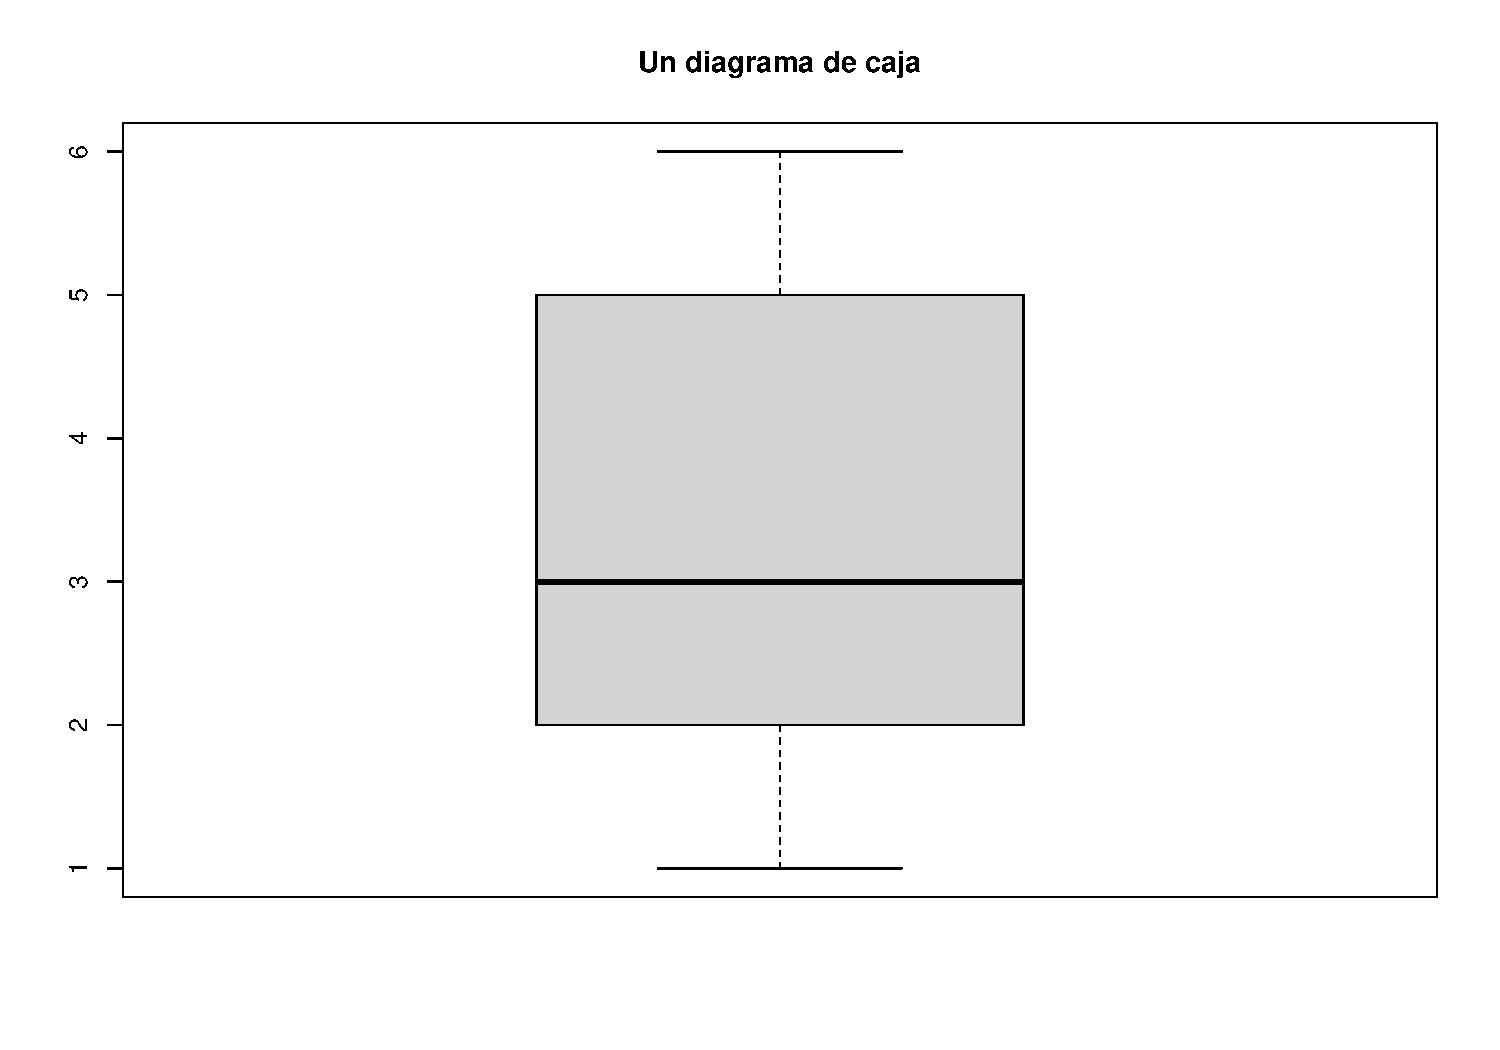
\includegraphics[width=250px]{Hora5_files/figure-beamer/unnamed-chunk-10-1} \end{center}
\end{frame}

\begin{frame}[fragile]{La función boxplot}
\protect\hypertarget{la-funciuxf3n-boxplot-1}{}
También podemos dibujar diversos diagramas de caja en un mismo gráfico.
De este modo, se pueden comparar con mayor facilidad:

\begin{Shaded}
\begin{Highlighting}[]
\FunctionTok{boxplot}\NormalTok{(dado,dados,dados2)}
\end{Highlighting}
\end{Shaded}

\begin{center}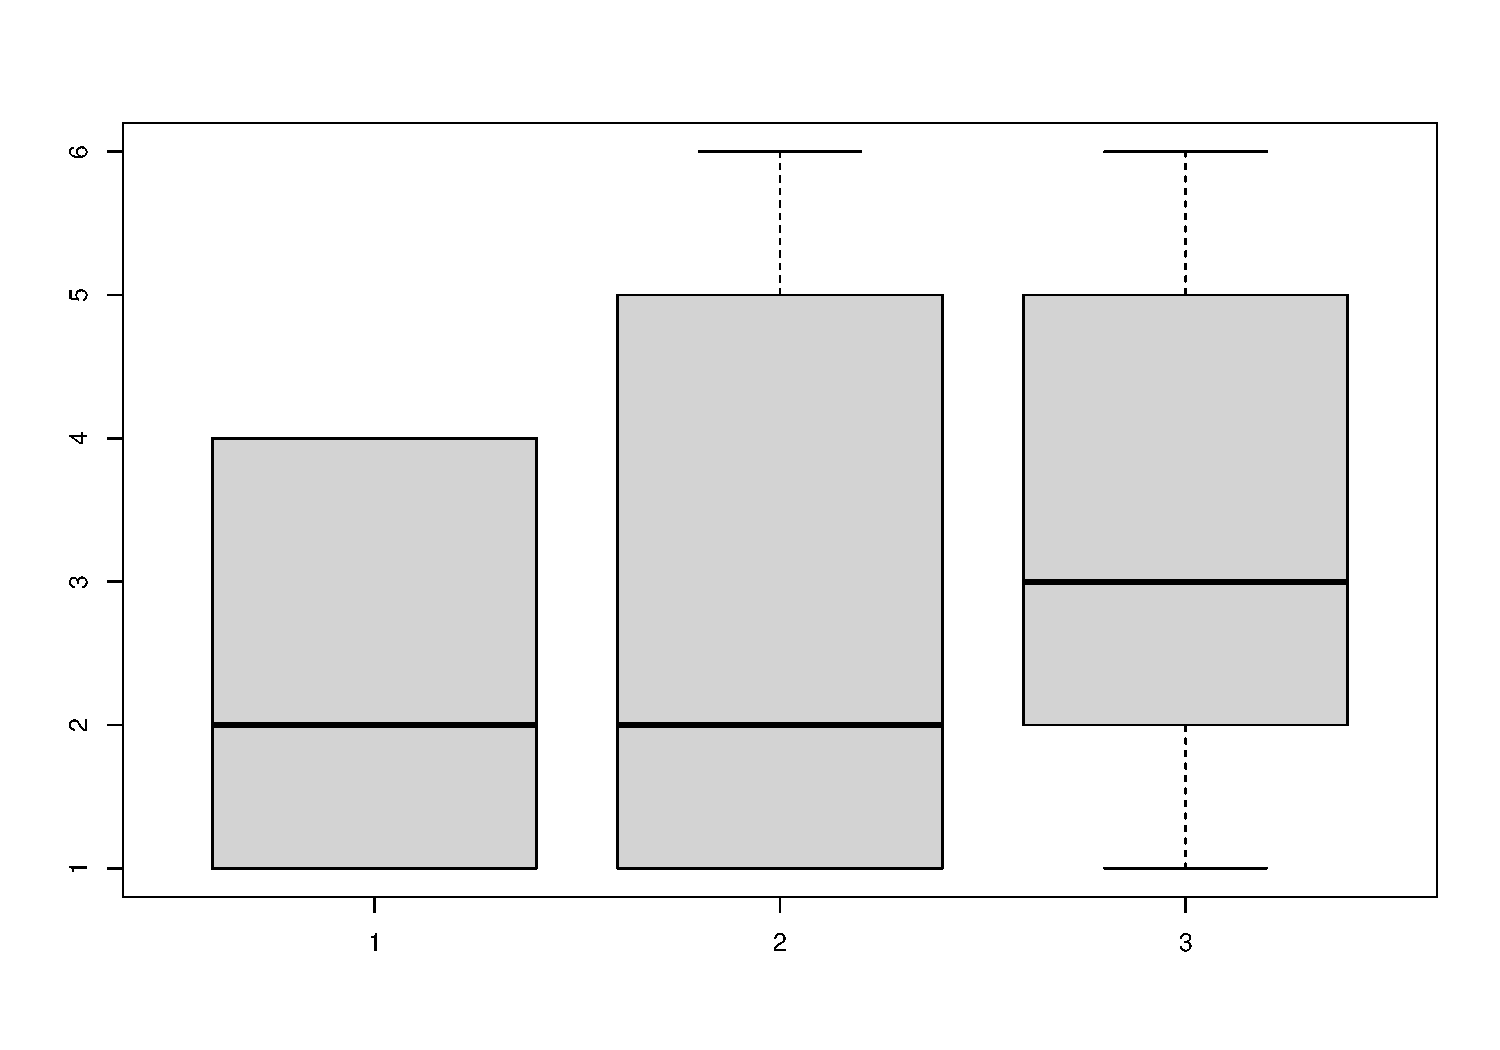
\includegraphics[width=250px]{Hora5_files/figure-beamer/unnamed-chunk-11-1} \end{center}
\end{frame}

\begin{frame}[fragile]{La función boxplot}
\protect\hypertarget{la-funciuxf3n-boxplot-2}{}
Además, podemos dibujar el diagrama de caja de todas las variables de un
data frame en un solo paso aplicando la instrucción
\texttt{boxplot(data.frame)}.

La mayoría de veces, dicho gráfico no será del todo satisfactorio.
Dibujar diagramas de factores no tiene sentido alguno. Estos gráficos se
pueden manipular incluyendo solo las variables de interés, cambiando los
nombres\ldots{}

Veamos un ejemplo:
\end{frame}

\begin{frame}[fragile]{Ejemplo 8}
\protect\hypertarget{ejemplo-8}{}
\begin{Shaded}
\begin{Highlighting}[]
\NormalTok{body }\OtherTok{=} \FunctionTok{read.table}\NormalTok{(}\StringTok{"../data/bodyfat.txt"}\NormalTok{, }\AttributeTok{header =} \ConstantTok{TRUE}\NormalTok{)}
\FunctionTok{boxplot}\NormalTok{(body)}
\end{Highlighting}
\end{Shaded}

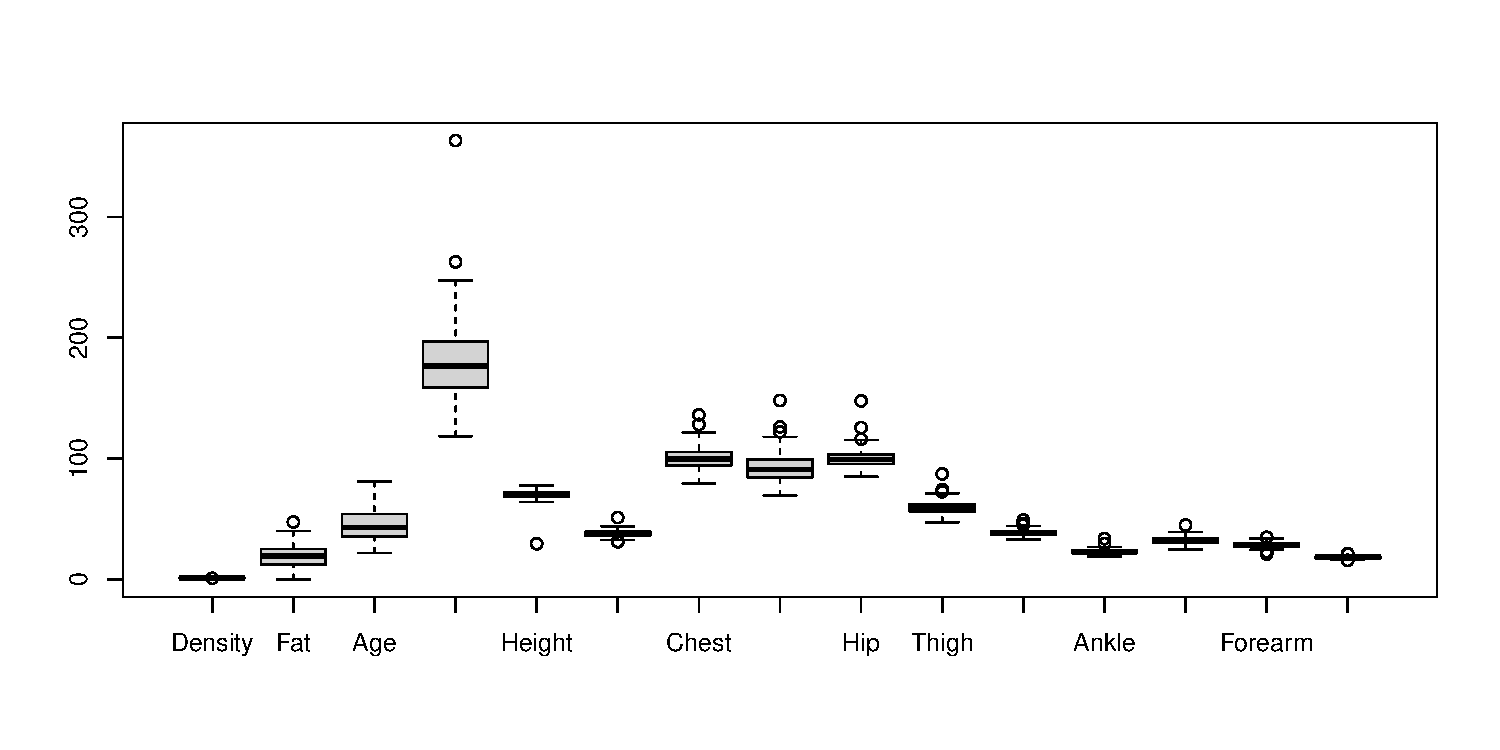
\includegraphics[width=0.8\linewidth]{Hora5_files/figure-beamer/unnamed-chunk-12-1}
\end{frame}

\begin{frame}[fragile]{Ejemplo 8}
\protect\hypertarget{ejemplo-8-1}{}
\begin{Shaded}
\begin{Highlighting}[]
\FunctionTok{boxplot}\NormalTok{(body[,}\DecValTok{7}\SpecialCharTok{:}\DecValTok{9}\NormalTok{], }\AttributeTok{names =} \FunctionTok{c}\NormalTok{(}\StringTok{"Pecho"}\NormalTok{, }\StringTok{"Abdomen"}\NormalTok{, }\StringTok{"Cadera"}\NormalTok{))}
\end{Highlighting}
\end{Shaded}

\begin{center}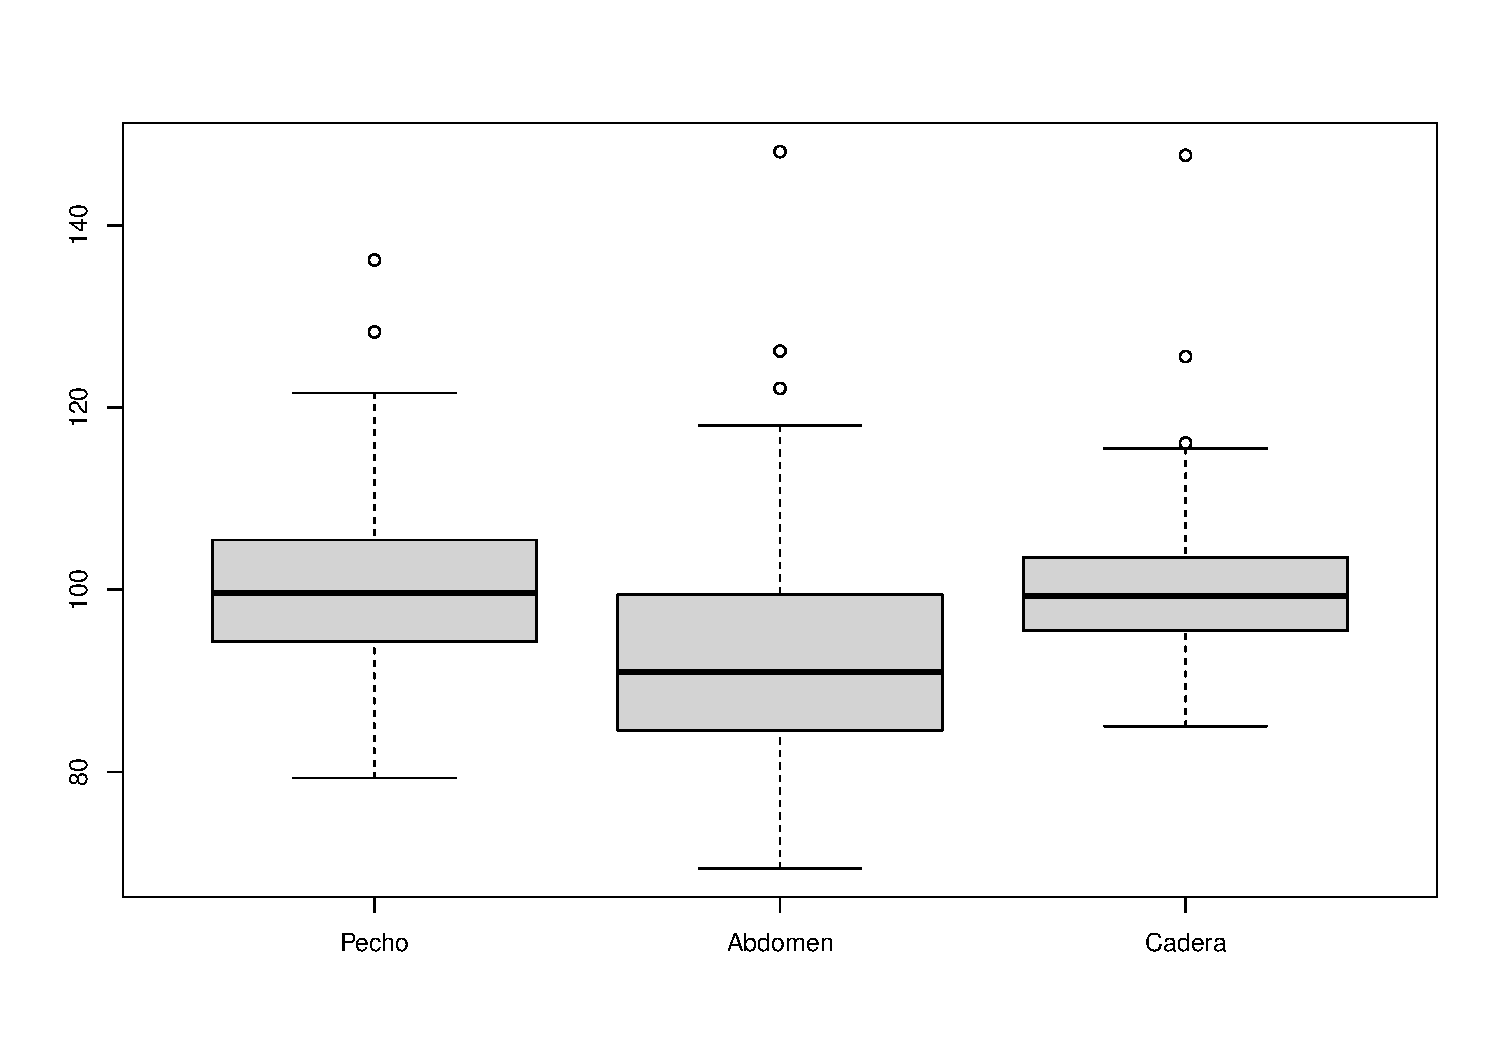
\includegraphics[width=275px]{Hora5_files/figure-beamer/unnamed-chunk-13-1} \end{center}
\end{frame}

\begin{frame}[fragile]{La función boxplot}
\protect\hypertarget{la-funciuxf3n-boxplot-3}{}
Agrupar varios diagramas de caja en un solo gráfico tiene por objetivo
poder compararlos visualmente, lo cual tiene sentido cuando las
variables tienen significados parecidos o cuando comparamos una misma
variable de poblaciones distintas.

La mayoría de las veces, querremos comparar diagramas de cajas de una
misma variable cuantitativa segmentada por los niveles de un factor.

La sintaxis de la instrucción para dibujar en un único gráfico los
diagramas de caja de una variable numérica de un data frame en función
de los niveles de un factor del mismo data frame es
\texttt{boxplot(var.numérica\textasciitilde{}factor,\ data\ =\ data\ frame)}
\end{frame}

\begin{frame}[fragile]{Ejemplo 9}
\protect\hypertarget{ejemplo-9}{}
\begin{Shaded}
\begin{Highlighting}[]
\FunctionTok{boxplot}\NormalTok{(circumference}\SpecialCharTok{\textasciitilde{}}\NormalTok{Tree, }\AttributeTok{data =}\NormalTok{ Orange, }\AttributeTok{ylab =} \StringTok{"Circunferencia del tronco (mm)"}\NormalTok{, }
        \AttributeTok{main =} \StringTok{"Boxplot de los naranjos en función del tipo de árbol"}\NormalTok{)}
\end{Highlighting}
\end{Shaded}

\begin{center}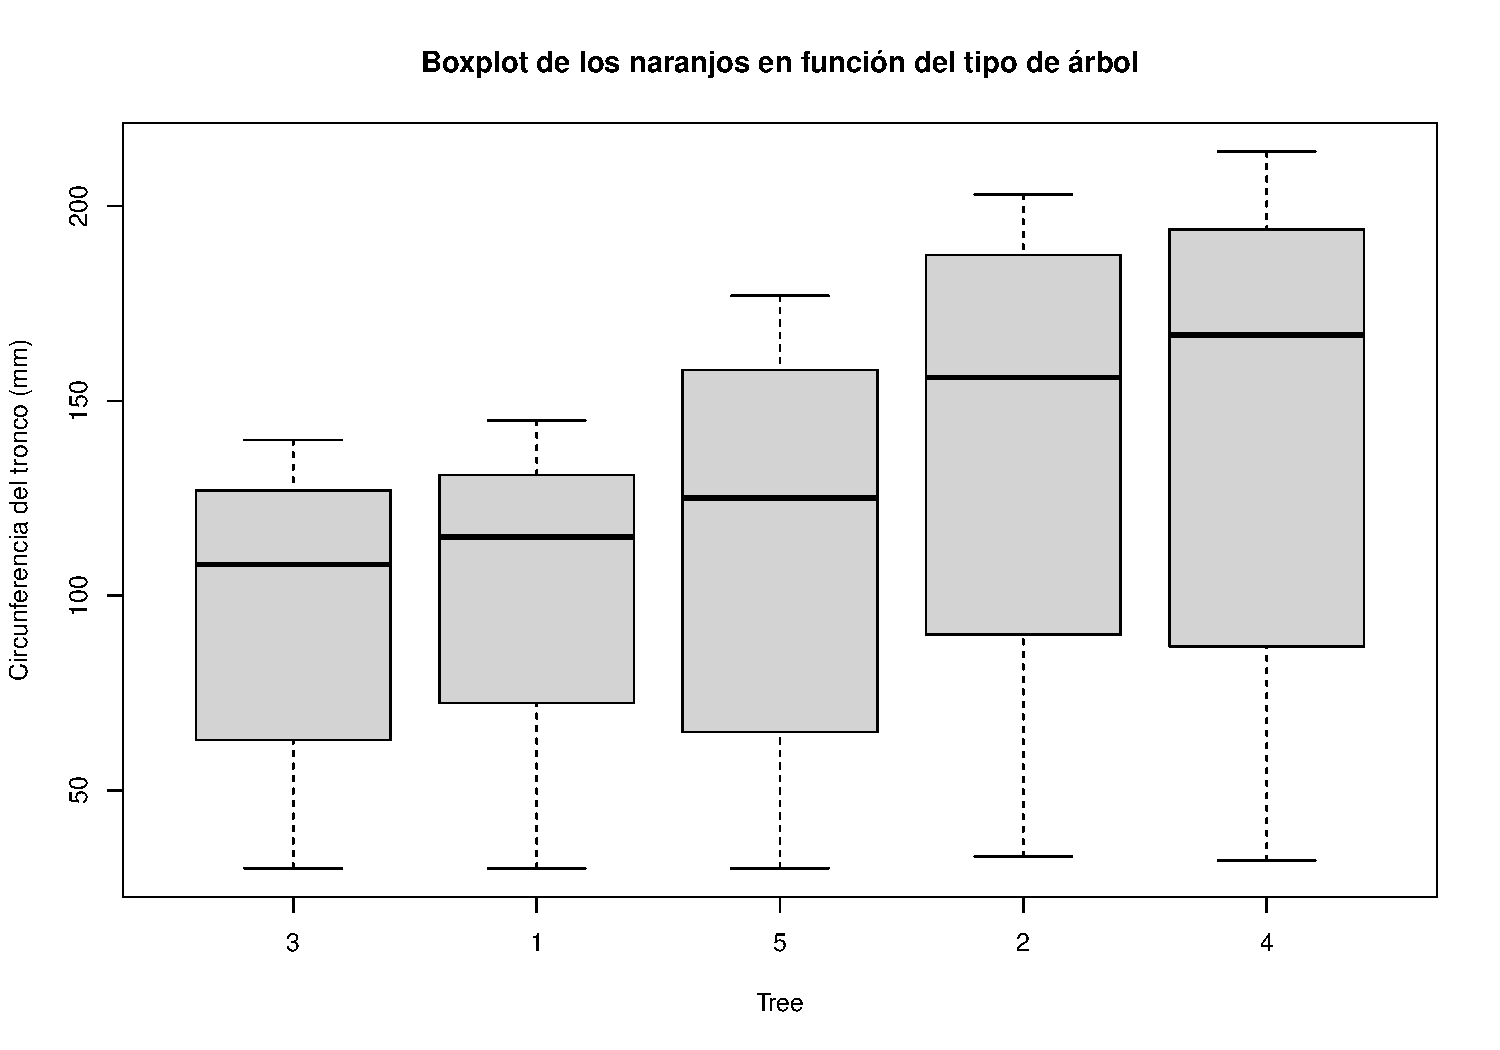
\includegraphics[width=250px]{Hora5_files/figure-beamer/unnamed-chunk-14-1} \end{center}
\end{frame}

\begin{frame}[fragile]{Parámetros de la función boxplot}
\protect\hypertarget{paruxe1metros-de-la-funciuxf3n-boxplot}{}
Todos los parámetros de la función \texttt{plot()} que tengan sentido
pueden ser utilizados en los argumentos de la función
\texttt{boxplot()}.

Aparte, la función \texttt{boxplot()} dispone de algunos parámetros
específicos, de los cuales mencionaremos:

\begin{itemize}
\tightlist
\item
  \texttt{notch} igualado a \texttt{TRUE} añade una muesca en la mediana
  de la caja. Si se da el caso en que las muescas de dos diagramas de
  cajas no se solapan, entonces con alto grado de confianza, concluimos
  que las medianas de las poblaciones correspondientes son diferentes.
\end{itemize}
\end{frame}

\begin{frame}[fragile]{Ejemplo 10}
\protect\hypertarget{ejemplo-10}{}
\begin{Shaded}
\begin{Highlighting}[]
\FunctionTok{boxplot}\NormalTok{(Sepal.Width}\SpecialCharTok{\textasciitilde{}}\NormalTok{Species, }\AttributeTok{data =}\NormalTok{ iris, }\AttributeTok{ylab =} \StringTok{"Anchura del sétalo (cm)"}\NormalTok{,}
        \AttributeTok{notch =} \ConstantTok{TRUE}\NormalTok{, }\AttributeTok{col =} \FunctionTok{c}\NormalTok{(}\StringTok{"cyan"}\NormalTok{,}\StringTok{"cyan2"}\NormalTok{,}\StringTok{"cyan4"}\NormalTok{),}
        \AttributeTok{main =} \StringTok{"Boxplot de iris"}\NormalTok{)}
\end{Highlighting}
\end{Shaded}

\begin{center}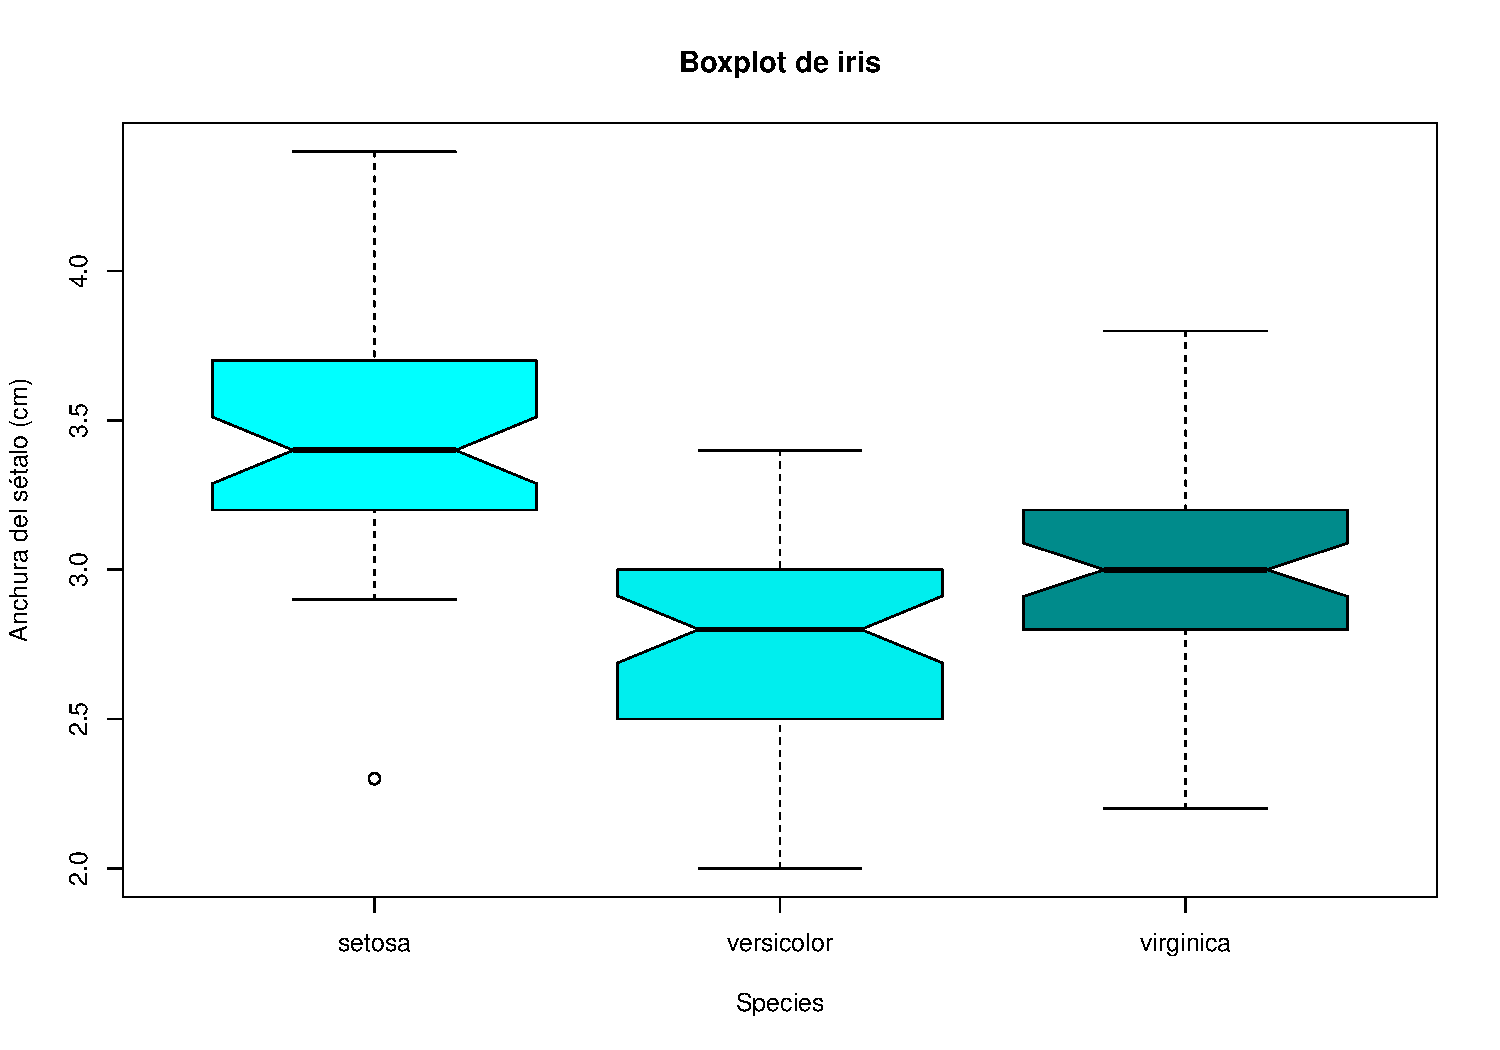
\includegraphics[width=250px]{Hora5_files/figure-beamer/unnamed-chunk-15-1} \end{center}
\end{frame}

\begin{frame}[fragile]{Ejemplo 10}
\protect\hypertarget{ejemplo-10-1}{}
Si quisiéramos marcar de alguna forma en un diagrama de caja, cosa que
puede ser muy útil en ocasiones, la media aritmética de la variable
correspondiente, podríamos hacerlo mediante la función \texttt{points}:

\begin{Shaded}
\begin{Highlighting}[]
\FunctionTok{boxplot}\NormalTok{(Sepal.Width}\SpecialCharTok{\textasciitilde{}}\NormalTok{Species, }\AttributeTok{data =}\NormalTok{ iris, }\AttributeTok{ylab =} \StringTok{"Anchura del sétalo (cm)"}\NormalTok{)}
\NormalTok{medias }\OtherTok{=} \FunctionTok{aggregate}\NormalTok{(Sepal.Width}\SpecialCharTok{\textasciitilde{}}\NormalTok{Species, }\AttributeTok{data =}\NormalTok{ iris, }\AttributeTok{FUN =}\NormalTok{ mean)}
\FunctionTok{points}\NormalTok{(medias, }\AttributeTok{col =} \StringTok{"pink"}\NormalTok{, }\AttributeTok{pch =} \DecValTok{15}\NormalTok{)}
\end{Highlighting}
\end{Shaded}

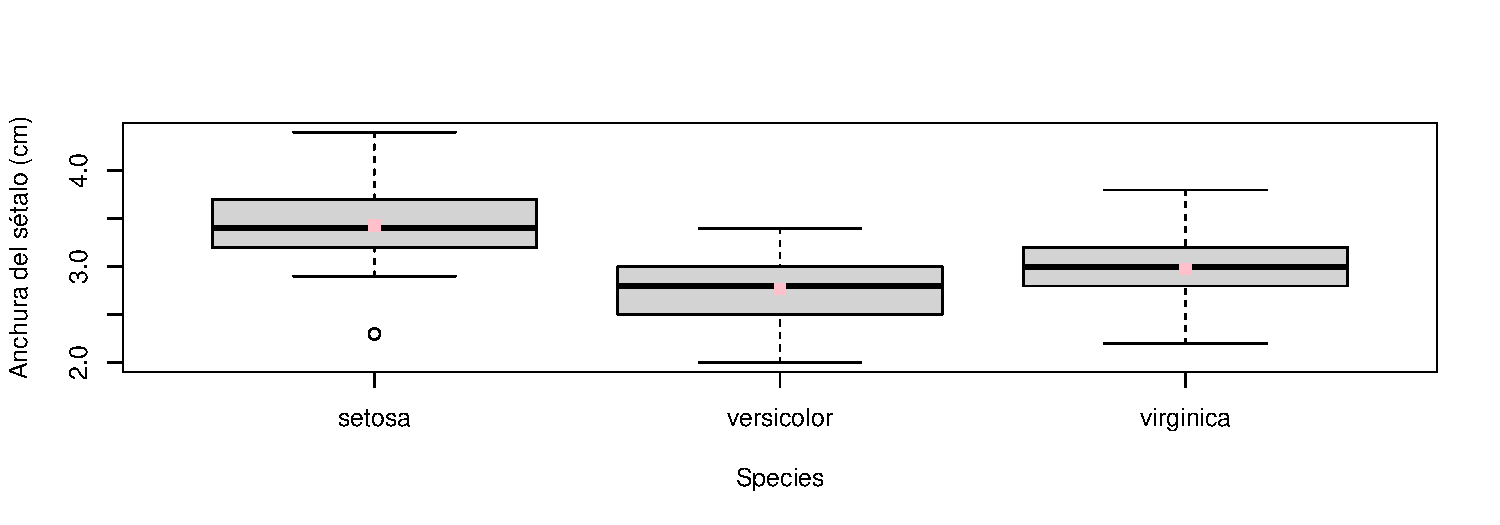
\includegraphics[width=0.8\linewidth]{Hora5_files/figure-beamer/unnamed-chunk-16-1}
\end{frame}

\begin{frame}{Ejemplo 10}
\protect\hypertarget{ejemplo-10-2}{}
La primera instrucción del chunk anterior genera el diagrama de cajas de
las anchuras de los sépalos en función de la especie. Por su parte, la
segunda instrucción lo que hace es calcular las medias aritméticas de
las anchuras según la especie. Finalmente, la tercera instrucción lo que
hace es añadir al diagrama un punto cuadrado a cada caja en la ordenada
correspondiente a su media aritmética.
\end{frame}

\begin{frame}[fragile]{La estructura interna de boxplot}
\protect\hypertarget{la-estructura-interna-de-boxplot}{}
Como ya sabemos, podemos estudiar la función interna de algunos objetos
con la función \texttt{str}.

Dicha función aplicada a un boxplot, nos produce una list. Podéis ver
esta list si introducís por consola la siguiente instrucción:
\texttt{str(boxplot(circumference\textasciitilde{}Tree,\ data\ =\ Orange))}
Destacaremos dos de sus componentes aquí:

\begin{itemize}
\tightlist
\item
  \texttt{stats} nos devuelve los valores
  \(b_{inf},\ Q_{0.25},\ Q_{0.5},\ Q_{0.75},\ b_{sup}\)
\item
  \texttt{out} nos retorna los valores atípicos. En caso de haber
  diversos diagramas en un plot, la componente \texttt{group} nos indica
  a qué diagramas pertenecen estos ouliers.
\end{itemize}
\end{frame}

\end{document}
